\documentclass[a4paper,14pt,russian]{report}
\usepackage[utf8]{inputenc}
\usepackage[T2A]{fontenc}
\usepackage{extsizes}
\usepackage{amsmath}
\usepackage{listings}
\usepackage{xcolor}
\usepackage{tabularx}
\usepackage{geometry}
\usepackage{titlesec}
\usepackage{graphicx}
\usepackage[font=small,labelfont=bf]{caption}
\usepackage{indentfirst}

\newcommand{\insertInstitute}{
  Институт компьютерных наук и технологий\linebreak
  Кафедра «Системный анализ и управление»
}
\newcommand{\insertTitle}{Последствия употребления MDMA}
\newcommand{\insertAuthor}{С А. Новиков}
\newcommand{\insertAuthorPosition}{студент гр 13532/1}
\newcommand{\insertVerifier}{А А. Ефремов}
\newcommand{\insertVerifierPosition}{доцент, кф.-м.н}

\newcommand{\sectionbreak}{\clearpage}
\newcommand{\subsectionbreak}{\clearpage}

\graphicspath{ {./images/} }
\renewcommand{\figurename}{Рисунок}
\renewcommand{\tablename}{Таблица}

\sloppy

\linespread{1.3}
\definecolor{lightgray}{gray}{0.95}
\renewcommand{\contentsname}{Содержание}
\renewcommand{\thesection}{\arabic{section}}
\newgeometry{left=3cm,right=2cm,top=2cm,bottom=2cm}
\setlength{\parindent}{1.25cm}
\lstset{
  backgroundcolor=\color{lightgray},
}


\begin{document}

\pagenumbering{gobble}
\begin{center}
  Министерство науки и высшего образования РФ\linebreak
  Санкт-Петербургский политехнический университет\linebreak
  Петра Великого\linebreak
  \insertInstitute\linebreak
\end{center}
\vspace{1.5cm}
\begin{tabularx}{\textwidth}{Xr}
  УДК $\rule{4cm}{0.15mm}$ & УТВЕРЖДАЮ \\
                           & $\rule{5cm}{0.15mm}$ \\
                           & $\rule{5cm}{0.15mm}$ \\
                           & $\rule{5cm}{0.15mm}$ \\
                           & «$\rule{0.8cm}{0.15mm}$» $\rule{2cm}{0.15mm}$ $\rule{1.1cm}{0.15mm}$ г. \\
\end{tabularx}
\vspace{1.5cm}
\begin{center}
  \insertTitle\par
\end{center}
\vspace{1.5cm}
\begin{tabularx}{1\textwidth}{Xll}
  \textbf{Выполнил:}    & & \\
  \insertAuthorPosition & $\rule{3.5cm}{0.15mm}$ & \insertAuthor \\
                        & подпись, дата & \\
  \textbf{Проверил:}      & & \\
  \insertVerifierPosition & $\rule{3.5cm}{0.15mm}$ & \insertVerifier \\
                          & подпись, дата & \\
\end{tabularx}
\vfill
\begin{center}
  Санкт-Петербург $\rule{1.1cm}{0.15mm}$ г.
\end{center}


\newpage
\pagenumbering{arabic}
\setcounter{page}{2}

\section*{Реферат}

\noindent Отчет 32 с., 3 рис., 2 табл., 4 источника. \\
MDMA, ЭКСТАЗИ, НАРКОТИК, ГАЛЛЮЦИНОГЕН, ФАРМАКОКИНЕТИКА \\
Объектом исследования является MDMA. \\
Цель работы - изучение влияния MDMA на человека. \\
В результате исследования были выписаны эффекты и последствия употребления MDMA.

\tableofcontents

\section{Введение}

Метиле́ндио́ксиметамфетами́н, MDMA, МДМА, 3,4-метилендиокси-N-метамфетамин — полусинтетическое психоактивное соединение амфетаминового ряда, относящееся к группе фенилэтиламинов, широко известное под сленговым названием таблетированной формы э́кстази (англ ecstasy, другие названия — Адам, XTC, E, X, Молли, Манди).

MDMA входит в число наиболее популярных наркотиков, особенно среди молодёжи, и получил заметное отражение в западной массовой культуре Распространён с 1980-х годов в среде рейв-культуры и завсегдатаев ночных клубов. Производство, хранение, транспортировка и распространение MDMA запрещены конвенцией ООН и являются уголовным преступлением в большинстве стран мира.

MDMA как психоактивное вещество действует сразу на несколько нейромедиаторных и нейрогормональных систем и усиливает переживания, как субъективно приятные, так и, в меньшей мере, неприятные. Он способен вызывать чувство эйфории, открытости и близости к другим людям при одновременном снижении страха и тревожности. Такие устойчивые эффекты, по мнению некоторых исследователей, выделяют MDMA среди других психостимуляторов и психоделиков в отдельную группу эмпатогенов. MDMA может усиливать депрессию, тревожность и другие негативные эмоциональные состояния. MDMA действует как стимулятор, хотя и не такой сильный, как амфетамины. Помимо рекреационного использования, до своего запрета MDMA использовался в качестве вспомогательного средства в психотерапии.

Согласно оценкам медиков, MDMA относится к группе низкоопасных рекреационных наркотиков, безопаснее алкоголя и табака Основным поводом для беспокойства является потенциальная нейротоксичность MDMA, продемонстрированная на животных, степень которой, однако, остаётся предметом дебатов. Наибольшая опасность связана с тем, что экстази могут принимать в сочетании с более вредными наркотиками. Считается, что длительное использование MDMA из-за нейротоксичности может приводить к понижению когнитивных способностей, проблемам с памятью, бессоннице, вспыльчивому и агрессивному поведению и расстройствам настроения и внимания, но эти вопросы не прояснены до конца. Кроме этого, приём MDMA может являться причиной появления такого синдрома, как длительное расстройство восприятия, вызванное галлюциногенами (HPPD). Очень редко приём MDMA может приводить к серьёзным медицинским последствиям, крайне редко — к смертельному исходу. Вопросы вреда и пользы MDMA и его легализации, полной или частичной, стали предметом длительной борьбы в «войне с наркотиками», сопровождавшейся моральной паникой, публичными и научными скандалами.

В XXI веке возобновились исследования MDMA как медицинского препарата для лечения серьёзных расстройств психики. Тем не менее, по состоянию на 2015 год MDMA не имеет утверждённых медицинских применений, и чтобы определить баланс рисков и пользы препарата, необходимы дополнительные исследования.

\section{История}

\subsection{Открытие и ранние исследования}

MDMA был впервые синтезирован при попытках найти новые средства для улучшения свёртываемости крови в 1912 году немецким химиком Антоном Кёлишем, работавшим на фармацевтическую компанию Merck, и запатентован в 1914 году как промежуточный продукт в синтезе кровоостанавливающего гидрастинина и его аналога метилгидрастинина.

Только около полувека спустя молекула MDMA вновь привлекает к себе внимание исследователей, уже в качестве психоактивного соединения — как родственное мескалину вещество Кратковременные исследования 1950-х — начала 1960-х годов по заказу армии США искали новые способы манипулирования сознанием и входили в знаменитую программу «МК Ультра», однако не были особенно успешными, их свернули после смерти одного из участников от передозировки MDA. Тогда MDMA на людях так и не был испытан.

Известность к MDMA пришла в конце 1970-х годов благодаря работам американского химика и исследователя психоактивных веществ Александра Шульгина В 1976 году по совету одной из своих студенток, Мари Клейнман, Шульгин синтезировал и испытал MDMA на себе, используя метод постепенного увеличения дозы.

\subsection{Применение в психотерапии}

Вскоре Шульгин, имевший хорошие связи в научном мире, знакомит с действием этого вещества более широкий круг учёных В первых научных статьях, посвящённых MDMA, вышедших в 1978 году, его действие на психику человека описано как «легко контролируемое изменённое состояние сознания с эмоциональными и чувственными оттенками».

\begin{figure}[!htb]
\centerline{
\includegraphics{shulgin}}
\caption{Александр Шульгин, 2010 г}
\end{figure}

Один из друзей Шульгина, психотерапевт Лео Зеф, ещё в 1977 году был поражён терапевтическим потенциалом MDMA и с энтузиазмом начал использовать его в практике Доктор Зеф способствовал распространению информации об открытии в среде психотерапевтов, особенно холистической и Нью Эйдж-направленности. Постепенно MDMA начал использоваться всё шире и шире как препарат, повышающий эффективность сеансов психотерапии.

В начале 1980-х годов MDMA применяют в клинической практике более тысячи врачей — по оценкам, до его запрета в США в психотерапевтических целях было использовано около полумиллиона доз вещества Зеф дал MDMA название «Адам», исходя из его «способности возвращать субъекта в состояние невинности, предшествовавшее возникновению чувства вины, стыда и собственной недооценки». Терапевты старались не привлекать к MDMA особенного внимания, поскольку никто не хотел повторения истории с ЛСД, запрещённым после его широкого распространения за пределы психотерапевтического применения.

\subsection{Распространение}

Вскоре употребление MDMA распространилось за пределы клинической практики, в особенности среди поклонников Нью Эйдж Начиная с середины 1970-х он начинает всё чаще встречаться в конфискованных образцах наркотиков, и к 1980 начинает преобладать над MDA.

С 1980-х начинается распространение MDMA в клубной субкультуре Особенно популярным и широко используемым он стал в Калифорнии и в Техасе, где MDMA распространялся в барах и ночных клубах Далласа и Форт-Уэрта. Название «Экстази» (англ. ecstasy, экстаз) придумал в 1981 году Майкл Клегг (англ. Michael Clegg), входивший в состав так называемой «техасской группы», начавшей в 1983 году легальное широкомасштабное производство MDMA для использования в рекреационных целях. По слухам, мировой популярности MDMA обязан активному распространению и пропаганде его сторонниками Ошо, которые завезли вещество в Нидерланды, где оно оставалось легальным до 1988. В Европе широкое клубное распространение экстази — рейвовое движение — берёт начало с Балеарских островов в 1986 году, и быстро охватывает весь мир.


\section{Механизм действия}

Действие MDMA наступает через 20—30 минут после перорального приёма и длится от часа и более, в зависимости от дозы Известно, что действие S-(+)-энантиомера MDMA более сильное, чем R-(-)-энантиомера: эффективные дозы для них составляют 80—120 мг и 300 мг соответственно. Это нетипично для психотомиметиков — обычно наоборот, большую психоактивность проявляют R-(-)-энантиомеры. Тем не менее, чаще всего вещество встречается и используется, в том числе в исследованиях по потенциальному применению в психотерапии, в виде рацемических смесей. Считается, что левовращающий R-(-)-изомер проявляет в большей степени психомиметические свойства (мескалиноподобные), а правовращающий S-(+)-изомер — стимулирующие (амфетаминоподобные).

\begin{figure}[!htb]
\centerline{
\includegraphics[width=0.5\textwidth]{formula}}
\caption{Энантиомеры MDMA, R-(-) — сверху, S-(+) — снизу}
\end{figure}

В отличие от других распространённых амфетаминов, MDMA в первую очередь влияет на механизмы нейрорегулирования серотонина — с преимущественным селективным действием на серотонинергические нейроны нигростриатной системы Серотонин является известным нейромедиатором, участвующим в регулировании многих высших функций сознания, а также настроения и ощущения удовольствия: у людей, испытывающих сильную депрессию, наблюдается пониженное количество серотонина. Проникая в нейроны головного мозга, вероятно, путём диффузии, MDMA, связываясь с белком-транспортировщиком серотонина SERT (K\textsubscript{d} 0,61 мкмоль, EC\textsubscript{50} 8 мкмоль), реверсирует его действие, так что вместо захвата отработавшего перенос возбуждения между нервными клетками серотонина снаружи и направления его обратно внутрь аксона для хранения, SERT начинает выкачивать серотонин из аксона в синапс — до 80\% всего доступного количества серотонина выходит в синаптическую щель, а затем рассеивается в межклеточной жидкости (в этом отношении MDMA в 10 раз превосходит метамфетамин). Этот эффект более характерен для S-(+)-энантиомера MDMA и связан с его психотропными свойствами. Помимо этого, MDMA связывается с белками, расщепляющими серотонин — MAOA и MAOB, ингибируя их активность (IC\textsubscript{50} 50 и 370 мкмоль, соответственно).

Однако эффект сильного выделения серотонина полностью не объясняет столь необычную психоактивность MDMA Точный механизм действия до конца не известен и является областью активных исследований. Дополнительно идентифицирован ряд нейроэффектов MDMA, следующих за выбросом серотонина или одновременно с ним, в том числе выделение таких нейромедиаторов, как дофамин (однако эффективность MDMA в этом отношении в 6 раз меньше, чем у метамфетамина), норадреналин (этот эффект частично ответственен за стимулирующие свойства MDMA, см. также раздел о стрессе) и ацетилхолин — MDMA напрямую воздействует, хотя и слабее, чем на сайт связывания серотонина, на a\textsubscript{2}- и a\textsubscript{1}-адренергические, M\textsubscript{1}- и M\textsubscript{2}-холинергические, H\textsubscript{1}-гистаминовые, b-, D\textsubscript{2}-, D\textsubscript{1}-рецепторы и серотониновые 5-HT\textsubscript{2A}-рецепторы синапсов (умеренные/слабые афинности, на крысах K\textsubscript{d} для a\textsubscript{2} 3,6, 5-HT\textsubscript{2A} 5,1, H\textsubscript{1} 5,7, M\textsubscript{1} 5,8, M\textsubscript{2} 15, a\textsubscript{1} 18, b 19, D\textsubscript{2} 95, D\textsubscript{1} 148  мкмоль, соответственно). Влияние MDMA на 5-HT\textsubscript{2A}-рецепторы связывают с галлюциногенными свойствами препарата, оно более характерно для его R-(-)-энантиомера (K\textsubscript{d} 3,3 μM). Эйфорические свойства MDMA, вероятно, частично связаны со стимуляцией им дофаминовых D2-рецепторов. Вообще большинство психологических эффектов скорее следуют фармакокинетике S-(+)-энантиомера, помимо этого, в результате метаболизма MDMA образуются другие вещества, в том числе известные психоактивные — MDA и другие, влияние которых на общий испытываемый эффект до конца не изучено.

Показано, что MDMA вызывает выделение гормонов — пролактина, вазопрессина и кортизола Лабораторные эксперименты на животных показали, что MDMA также активирует окситоциновые нейроны гипофиза, в основном за счёт стимуляции 5-HT\textsubscript{1A} рецепторов. В некоторых экспериментах оказывается, что эффект эмпатии, вызываемый MDMA, напрямую связан с выделением «гормона привязанности» окситоцина. Дружелюбность людей под воздействием MDMA оказалась прямо темпорально скоррелированной с уровнем окситоцина, а его выброс оказался связанным с внешней температурой — чем она выше, тем сильнее высвобождение окситоцина (что повышает этот эффект в клубах). Есть, однако, и работы, оспаривающие связь эффекта эмпатии от MDMA с окситоцином. Хотя кортизол влияет на передачу нервного сигнала и память (см. тут), связь его выброса с субъективными эффектами приёма MDMA не ясна, так как предварительный приём ингибитора синтеза кортизола метирапона блокирует рост концентрации гормона в крови после приёма MDMA, не изменяя ухудшения памяти и изменения настроения под влиянием MDMA.

Исследования указывают на то, что прекращение действия MDMA связано не с выведением вещества из организма или его превращением, а с развитием толерантности к его наличию в организме Изменение уровня серотонина под действием MDMA имеет сложную форму: после первоначального выброса его концентрация через несколько часов, по окончании начального периода действия вещества, падает ниже нормы, затем через сутки вырастает до обычных значений, а потом падает на несколько дней. Этот последний провал уровня серотонина вызывается в частности тем, что какие-то продукты метаболизма MDMA являются необратимым ингибитором триптофан-гидроксилазы — фермента, ответственного за синтез серотонина (сам MDMA in vitro такого эффекта не проявляет). Активность энзима в мозге существенно падает на несколько часов, но при этом не восстанавливается до исходной даже через несколько недель после приёма MDMA. Кроме того, использование MDMA способно вызывать долгосрочное — месяцы и годы после последнего приёма — угнетение системы серотонинопроизводящих нейронов в лабораторных животных, выраженность которого растёт с возрастом животных — это связывают с его нейротоксичностью.

\section{Фармакокинетика}

Действие MDMA характеризуется сложно-нелинейной фармакокинетикой, связанной с различными скоростями метаболизирования стереоизомеров: S-(+)-энантиомер является более активным. Увеличение дозы и/или более частое употребление непропорционально быстро увеличивает содержание MDMA в плазме крови, поэтому при приёме больших доз вещества значительно повышается риск оксидативного стресса, вызываемого метаболитами MDMA — HHMA и HHA.

Максимальная концентрация MDMA в крови достигается между 1,5—2 часами после орального приёма и составляет для типичной дозы в 100 мг MDMA около 200 мкг/л. Основным местом всасывания вещества служит, вероятно, тонкий кишечник, а внутри организма путём транспортировки MDMA является простая диффузия — как слабое основание (pKa около 9,9) невысокой молекулярной массы вещество легко проходит через клеточные мембраны. После этого MDMA метаболизируется и медленно выводится из организма, — при этом для типичных доз уровень вещества в крови понижается до половины пиковой концентрации примерно через 7—8 часов после пика (после приёма 100 мг рацемической смеси для S-(+)-MDMA это время составляет 4,8 ч, а для R-(-)-MDMA — 14,8 ч, для 40 мг — 3,6 ч и 5,8 ч, соответственно). Основной путь очистки организма от MDMA — разрушение в печени под действием цитохромов P450, с мочой за 36 часов выводится в неизменном виде лишь 3—8\% исходного количества препарата (по другим данным — около 20\%). Распределение MDMA по организму, по-видимому, неоднородно, с наибольшими концентрациями в головном мозгу и печени, однако оно исследовалось только на погибших от передозировки и демонстрирует сильные индивидуальные различия, поэтому результаты должны приниматься с осторожностью.


Схема основных путей метаболизма MDMA, направо уходит N-деметилирование, налево — окислительное деалкилирование. Рядом со стрелками указаны ферменты, вызывающие реакции, CYP — цитохромы P450, COMT — катхол-О-метилтрансфераза. MDA также обладает психоактивным действием, HHMA и HHA токсичны для клеток печени и нейронов, а также вызывают оксидативный стресс
Сейчас известно о четырёх различных путях метаболизма MDMA: N-деметилирование, окислительное деалкилирование, дезаминирование и присоединение метильного, глюкуронового или сульфатного остатков. Основные из них — первые два, соотносящиеся по скорости примерно как 1:10 и идущие в основном в печени под действием цитохромов P450. Окислительное деалкилирование в основном (примерно на 30\%) обеспечивается цитохромом P450 2D6 (CYP2D6), другие вносящие вклад ферменты: CYP1A2, CYP2B6 и CYP3A4. Продуктом N-деметилирования являются психоактивные метаболиты, включая MDA. Этот метаболический путь обеспечивается в основном ферментом CYP2B6 системы цитохрома P450, и в меньшей степени CYP2D6, CYP1A2 и CYP3A4.

Одна из причин фармакокинетической нелинейности метаболизма MDMA заключается в ингибировании CYP2D6 и CYP2D8 молекулами MDMA путём образования комплексов. Одна стандартная доза MDMA (75 мг) приводит к понижению активности CYP2D6 на 75\% в течение часа, и даже через двое суток активность составляет всего лишь 50\% от исходной, полностью восстанавливаясь только через срок до 10 дней. В результате использование MDMA чаще, чем раз в неделю, увеличивает достигаемые максимальные концентрации в крови.

Известно, что цитохромы P450 демонстрируют широкий генетический полиморфизм, и их эффективность может сильно варьироваться — что в принципе должно оказывать влияние на метаболизм MDMA, но работ, посвящённых исследованию этого эффекта, по состоянию на 2014 год не проводилось.

Идентифицированные метаболиты MDMA включают MDA (3,4-метилендиоксиамфетамин или тенамфетамин, который единственный надёжно обнаруживается в крови и плазме), HMMA (4-гидрокси-3-метокси-метамфетамин), HMA (4-гидрокси-3-метоксиамфетамин), DHA (3,4-дигидроксиамфетамин или альфа-метилодопамин), MDP2P (3,4-метилендиоксифенилацетон), MDOH (N-гидрокси-3,4-метилэнидиосидамфетамин) и другие. Метаболиты MDMA, в свою очередь, в основном подвергаются воздействию цитохромов P450, катехол-О-метилтрансферазы, глюкуронированию или сульфированию.

Катехол-О-метилтрансфераза, которая разрушает катехоламины, также демонстрирует генетический полиморфизм, влияющий на её активность. Хотя этот фермент не участвует в метаболизме самого MDMA, он разлагает ядовитые продукты его превращения. Исследования на людях показывают, что низкоактивный вариант фермента существенно влияет на выведение HHMA и HHA с мочой (оно увеличивается двукратно). В исследованиях на культурах клеток печени человека показано, что индуцированная MDMA гепатотоксичность существенно выше для культуры с низкоактивным вариантом фермента.

Полярные гидроксилированные продукты метаболизма выводятся из организма с мочой: основной обнаруживаемый там метаболит — HMMA (более 20\% исходной дозы), следующий — ННМА, а выводимый MDA составляет менее 10\% от исходного MDMA. Точный вклад каждого из этих веществ в общий эффект до конца не изучен. Также остаётся открытым вопрос токсичности каждого из этих метаболитов. Известно что MDA, MDP2P и MDOH являются отдельными психоактивными веществами.

\section{Взаимодействие с другими веществами}

Известно, что препараты, ингибирующие активность цитохрома P450 2D6, например ритонавир, увеличивают максимальную концентрацию MDMA в крови, что однако, приводит к ослаблению желательных эффектов приёма MDMA и усиливает его побочные эффекты.

Так как и метамфетамин, и MDMA метаболизируются одним и тем же цитохромом P450 2D6, при совместном применении они ингибируют его ещё сильнее, что приводит к синергетическому эффекту увеличения концентраций обоих веществ в крови, подтверждённому на крысах и in vitro, и, по-видимому, повышает суммарную токсичность — некоторые случаи медицинских осложнений от приёма MDMA были связаны с последующим употреблением других амфетаминов.

Взаимодействие с кофеином исследовалось на крысах, обнаружено, что совместное применение кофеина и MDMA сильнее повышает температуру тела у крыс по сравнению с отдельными препаратами.

Приём экстази одновременно с препаратами, ингибирующими обратный захват серотонина или моноаминоксидазу, к которым относятся некоторые современные антидепрессанты, может вызвать внезапный острый серотониновый синдром — угрожающее жизни состояние, требующее неотложной медицинской помощи с использованием антисеротониновых препарато. С другой стороны, приём СИОЗС пароксетина за трое суток до введения MDMA серьёзно подавляет психологические и физиологические эффекты наркотика, несмотря на увеличение его максимальной концентрации в крови примерно на 20—30\%. Аналогичное действие проявляют СИОЗС циталопрам и флуоксетин, а также блокаторы выброса норадреналина ребоксетин и дулоксетин.

В исследованиях на крысах введение силденафила (виагры) сразу перед введением MDMA и за сутки до него снижало эффект последующего угнетения 5-HT системы нейронов без изменений в гипертермическом ответе и скорости метаболизма MDMA Аналогичный нейропротекторный эффект показан на крысах на варденафиле и миноксидиле и предполагается для других ингибиторов фосфодиэстеразы 5 (ФДЭ-5) — возможный механизм действия включает увеличение производства цГМФ, активацию протеинкиназы G (PKG) и открытие митохондриальных АТФ-чувствительных калиевых каналов, что подтверждается аналогичным эффектом от введения аналога цГМФ, 8-бромгуанозин цикло-3′,5′-монофосфата, и блокированием эффекта нейропротекции ингибиторами PKG и блокираторами калиевых каналов. Таким образом, предположительно, сочетанное употребление MDMA и препаратов для улучшения эрекции, аналогичных по механизму действия силденафилу, может снижать нейротоксичность MDMA.

Также на крысах нейропротективные эффекты при одновременном введении с MDMA демонстрируют: геминейрин (даже в условиях гипертермии), 2-дезокси-D-глюкоза (только при отсутствии гипертермии), хлорфенамин и дифенгидрамин (димедрол), тетрагидроканнабинол, антиоксиданты ацетилцистеин, цистеин, витамин C, липоевая кислота, прекурсоры серотонина триптофан и 5-гидрокситриптофан, блокатор выброса дофамина мазиндол, блокаторы выброса норадреналина ребоксетин и дулоксетин, антагонист 5-HT2A-рецепторов кетансерин: 868, специфический ингибитор моноаминоксидазы типа Б (ИМАО) селегилин и селективные ингибиторы обратного захвата серотонина (СИОЗС), такие как флуоксетин, циталопрам и пароксетин. Обратный эффект демонстрируют никотинамид, мепирамин и трипеленнамин, недостаток витамина E (также усиливает гепатоксичность).

На крысах гипертермию от воздействия MDMA подавляют препараты-антагонисты 5-HT2A-рецепторов, например кетансерин, рисперидон, миртазапин (при введении до и после MDMA), СИОЗС флуоксетин (но только при предварительном введении, ранние работы не находили этого эффекта, антипсихотики рисперидон и галоперидол, неселективный антагонист адренергических рецепторов карведилол (у людей он же, принятый за час до MDMA, в лабораторных условиях подавляет гипертермию, повышение кровяного давления и частоты сердцебиения, не влияя на субъективные эффекты MDMA) У клубных танцоров наблюдаемая гипертермия оказалась положительно скоррелированной с курением табака и отрицательно — каннабиса.

Приём алкоголя или каннабиса вместе с MDMA, по-видимому, не показывает взаимного влияния на фармакокинетику и психологические эффекты этих веществ, за возможным исключением удлинения эйфории и приятных ощущений от алкоголя и MDMA Совместный приём GHB и MDMA усиливает эйфорический эффект и уменьшает среднесрочные отрицательные постэффекты. Галоперидол уменьшает улучшение настроения под действием MDMA и маниакальность, не оказывая влияния на другие психологические параметры и скорость сердцебиения.

\section{Эффекты при употреблении}

\subsection{Предсказуемость и временное развитие эффектов}

Сравнение концентрации MDMA в крови и вызываемых им субъективных эффектов после орального приёма дозы в 1,6 мг/кг тела Синяя кривая даёт среднюю концентрацию, область вокруг неё — стандартное отклонение. Красная кривая даёт силу субъективных эффектов — видна краткосрочная толерантность организма.

\begin{figure}[!htb]
\centerline{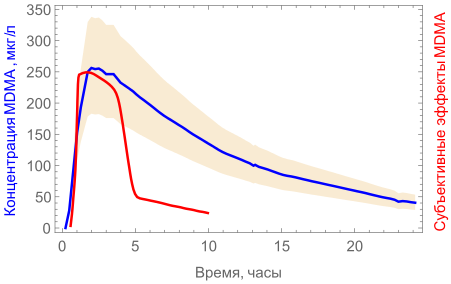
\includegraphics{effects}}
\caption{Сравнение концентрации MDMA в крови и вызываемых им субъективных эффектов после орального приёма дозы в 1,6 мг/кг тела}
\end{figure}

Воздействие MDMA на организм отличается как от стимуляторов, так и от галлюциногенов. В отличие от последних, оно намного более предсказуемо (что подтверждается двойными слепыми исследованиями) и имеет определённые фазы, зависит от дозы, эмоционального и физического состояния человека, а также толерантности организма. Среди всей семьи близкородственных эмпатогенов MDMA, как считается, вызывает наиболее субъективно приятные эффекты, что является причиной его неизменной популярности на рынке синтетических наркотиков.

Обычно первые эффекты проявляются в течение 30—60 минут после перорального введения, достигая пика через 75—120 минут Затем следует фаза плато (англ. plateau), которая длится приблизительно 3,5 часа и заканчивается возвращением субъективных показателей к исходным значениям. Для продления желательных эффектов некоторые пользователи принимают дополнительные таблетки экстази либо сразу (на слэнге это называется «складированием» — англ. stacking) либо во время плато, растягивая таким образом эффект («бустинг» — англ. boosting). Клинические проявления употребления экстази могут значительно варьировать, так как дозировка MDMA, а также состав примесей, в том числе психоактивных, меняются от таблетки к таблетке в широких пределах.

\subsection{Физиологические эффекты}

MDMA возбуждает симпатическую нервную систему и приводит к некоторым проявлениям серотонинового синдрома, с которым и связывается его физиологическое действие. Возможно, перевозбуждению способствует и атмосфера клубов с громкой музыкой, световыми шоу и плотными толпами. На гормональном уровне MDMA вызывает выброс кортизола, пролактина, окситоцина и вазопрессина.

MDMA вызывает стимуляцию сердечно-сосудистой системы: в дозах от 1 мг/кг наблюдаются повышение артериального давления, ускорение сердцебиения и увеличение минутного объёма крови. В рандомизированном двойном слепом плацебо-контролируемом исследовании приём 125 мг MDMA приводил к повышению систолического и диастолического давления примерно на 25 мм ртутного столба, и к увеличению пульса примерно на 25 ударов в минуту (плацебо — примерно 7 и 10, соответственно).

Под воздействием MDMA изменяется нормальный процесс терморегуляции — сужаются капилляры кожи и затрудняется потоотделение при одновременном резком усилении производства тепла в мозгу. Это многократно усиливает опасность перегрева (либо переохлаждения — в условиях низкой температуры). Даже при отсутствии физических нагрузок, в лабораторных условиях, приём MDMA в количестве 1,5—1,7 (2) мг на кг массы тела приводит к повышению температуры на 0,3—0,5 °C (0,4—2,0 °C, соответственно). Полевые исследования танцоров в клубах показали ещё более высокие значения: повышение внутренней температуры на 1,1 °C и температуры кожи на 1,8 °C.

Также под воздействием MDMA (и амфетаминов) у животных нарушается проницаемость гемато-энцефалического барьера, что приводит к переходу воды и ионов натрия из крови в мозговую межклеточную жидкость, приводя к гипернатриемии мозга, тесно скоррелированной со степенью повышения температуры тела. Это является фактором риска, дополнительно способствующим периферийной гипонатриемии как следствию неумеренного потребления воды под действием ощущаемой жажды и уменьшения потоотделения (в результате спазма капилляров кожи) и диуреза (в результате выброса вазопрессина).

MDMA вызывает мидриаз — расширение зрачков, причём этот эффект скоррелирован с концентрацией MDMA в крови и продолжается дольше психологических эффектов. Также действие MDMA ухудшает реакцию зрачков на свет — замедляет её и снижает её величину, этот эффект скоррелирован с психологическими эффектами препарата и проявляет такую же краткосрочную толерантность. В больших дозах MDMA вызывает косоглазие в виде эзофории.

Характерными побочными физиологическими эффектами MDMA являются тризм — спазм жевательной мускулатуры, и связанный с ним и перевозбуждением бруксизм — скрежет зубами.

\subsection{Психологические эффекты}

\subsubsection{Общий обзор психологических эффектов}

MDMA в целом вызывает эйфорию, однако его действие глубже и сопровождается разнообразными психологическими эффектами. Как показывают исследования, MDMA может усиливать любое настроение, в том числе негативное, и его эффект зависит от внутренних ожиданий и окружения принимающего.

Результаты воздействия также варьируются в зависимости от дозы: в двойных слепых лабораторных испытаниях в дозировке 0,5 мг/кг эффекты MDMA не прослеживаются, а при повышении дозировок в таблетках экстази субъективно положительные эффекты нарастают примерно до дозы в 80—100 мг, а затем начинают спадать на фоне усиливающихся субъективно отрицательных и полностью пропадают при дозировке около 180 мг.

\begin{table}[!htb]
\centering
\caption{Частота субъективных клинических проявлений при употреблении MDMA}
\label{table:effects}
\begin{tabular}{|l|l|}
  \hline
  Признак                              & Частота, \% \\
  \hline
  Ощущение «близости» с другими людьми & 90 \\
  Тризм                                & 75 \\
  Тахикардия                           & 72 \\
  Сухость во рту                       & 61 \\
  «Люминесценция» объектов             & 42 \\
  Тремор                               & 42 \\
  Затруднения в концентрации внимания  & 38 \\
  Потливость                           & 38 \\
  Парестезия                           & 35 \\
  Ощущение озноба или жара             & 33 \\
  Бессонница                           & 31 \\
  Повышенная чувствительность к холоду & 27 \\
  Головокружение                       & 24 \\
  Пониженное настроение                & 21 \\
  Зрительные галлюцинации              & 20 \\
  Нарушения зрения («смазанность»)     & 20 \\
  Головная боль                        & 17 \\
  Беспокойство, страх                  & 12 \\
  \hline
\end{tabular}
\end{table}

Принимающие экстази обычно описывают своё внутреннее состояние как эйфорию, интимность и близость к другим людям — «все люди — мои друзья»; ощущение «полёта, бесконечного счастья, высокой чувствительности» (см. таблицу \ref{table:effects}). В период действия MDMA повышается самоуверенность, настроение, мнительность, экстравертированность, наблюдается ускорение ассоциативных процессов, повышенная чувствительность (зрения, слуха, осязания), бодрость и эмоциональное возбуждение. Некоторые пользователи могут испытывать состояние ошеломлённости, нарушения восприятия и/или расстройства самовосприятия, изменения восприятия времени и пространства, мании, сбои в мышлении, страхи потерять контроль над телом и разумом, галлюцинации и псевдогаллюцинации, синестезию, изменения в восприятии, обостряется память и/или воображение.

\subsubsection{Влияние на настроение, социальность и эмпатию}

Действие MDMA на настроение может быть очень сильным — в исследовании 2003 года 91\% британских пользователей отмечали возникновение эйфорической волны (англ euphoric rush) после приёма экстази. Некоторые интервьюируемые отмечали, что воздействие экстази превосходит любые приятные ощущения, которые они испытывали в жизни, в то время как другие начинающие пользователи, наоборот, указывали, что воздействие оказалось не таким приятным, как они ожидали.

Повышение настроения, дружелюбности и энергичности после приёма около 100 мг MDMA подтверждается в плацебо-контролируемых лабораторных исследованиях. Характерна эмоциональная открытость, чувство сопричастности и близости к окружающим, сопровождающиеся желанием разговаривать и обсуждать свои ощущения. В памятках по обращению с людьми подчёркивается общая кооперативность и отсутствие агрессии у лиц, находящихся под влиянием экстази, а отдельные свидетельства полиции Англии о рейвах первого поколения — с широким распространением только экстази без других наркотиков, включая алкоголь — указывают на меньшее число правонарушений по сравнению с другими сборищами людей такого же масштаба.

Объективные измерения в плацебо-контролируемых лабораторных исследованиях показывают диапазон результатов влияния на когнитивную эмпатию от неизменности распознавания эмоций до улучшения распознавания положительных эмоций на фоне снижения распознаваемости отрицательных с тенденцией к усилению эффекта при переходе от доз 0,75 мг/кг к 1,5 мг/кг. Эмоциональная эмпатия (степень сопереживания) от MDMA увеличивается, так же как и щедрость, воспринимаемая позитивность социального взаимодействия и стремление к социализации (в том числе у лабораторных животных), а степень распознавания социального отвержения и его воздействие на самооценку снижается.

Менее широко известно, что в лабораторных и полевых исследованиях оказывается, что MDMA усиливает и отрицательное настроение: в лабораторных условиях показано усиление депрессии, страха перед будущим, тревожности и чувства одиночества, причём эти эффекты сильнее выражены среди женщин. Возможно, что такое отрицательное влияние на настроение, более характерное для лабораторных исследований, связано с повышением ценности социального взаимодействия под действием MDMA: в то время как в лаборатории социальные взаимодействия ограничены, в обычных условиях приём экстази происходит в компаниях или толпах. В полевых условиях пользователи экстази отмечают иногда возникающие внезапные приступы тревожности, паники, чувства потери контроля и перевозбуждения, причём они могут возникать одновременно с позитивными ощущениями или чередоваться с ними во время действия MDMA.

\subsubsection{Расстройства восприятия}
MDMA, особенно в высоких дозах, вызывает лёгкие расстройства восприятия в виде рудиментарных галлюцинаций, усиления яркости и чёткости предметов, трёхмерного восприятия двумерных объектов, микро- и макропсий и чувства изменений в себе и окружающем, которые обычно воспринимаются субъективно положительно. Вариации частоты встречаемости галлюцинаций простираются в различных исследованиях от «редких» до 43\% респондентов.

\subsubsection{Сексуальная функция}
Стимулирующее влияние MDMA на сексуальную функцию неясно, однако ретроспективные опросы употребляющих указывают на тот же или пониженный уровень либидо, но с обострением чувственного удовольствия от секса. В то же время отмечается усложнение достижения сексуального возбуждения и оргазма, особенно мужчинами, что, возможно, связано с выбросом пролактина под действием MDMA. Также в прямых лабораторных экспериментах MDMA вызывает похожие эффекты и снижение сексуальной активности у крыс.

\subsection{Побочные действия}

\begin{table}[!htb]
\centering
\caption{Статистический риск смерти от употребления MDMA, алкоголя и табака по Великобритании, 2006}
\label{table:deaths}
\begin{tabular}{|l|l|l|l|}
  \hline
  Вещество & Смертей & Употребляющих & Процент смертности \\
  \hline
  Никотин  & 114 тыс & 12,5 млн      & 0,912 \% \\
  Алкоголь & 22 тыс  & 58 млн        & 0,038 \% \\
  MDMA     & 33      & 800 тыс       & 0,004 \% \\
  \hline
\end{tabular}
\end{table}

Побочные действия MDMA сходны с другими стимуляторами амфетаминового ряда и включают в себя: излишне повышенный тонус мышц, повышение артериального давления (обычно как после физических нагрузок средней силы), тризм жевательной мускулатуры (сложности при раскрытии рта), бруксизм (скрежет зубами), акатизию (невозможность усидеть на месте), реже — сухость во рту, бессонницу, головную боль, головокружение, тошноту, снижение аппетита, смазанность зрительного восприятия. Редко при приёме экстази — около 1 случая на 10 000 принимаемых таблеток — встречаются серьёзные осложнения, с которыми пользователи обращаются в больницы, очень редко — около 1 на 1 800 000 таблеток — со смертельным исходом (см. таблицу \ref{table:deaths}), при лабораторных исследованиях MDMA на добровольцах (более 1100 человек к 2016 году) серьёзных медицинских осложнений, требующих госпитализации, не наблюдалось ни разу. После прохождения плато в течение нескольких дней характерные жалобы включают в себя боль и «зажатость» мышц, понижение внимания и настроения, тревожность, ухудшение сна и бессонницу.

\section{Толерантность}
MDMA характеризуется как кратковременной толерантностью, формируемой в организме после однократного использования и продолжающейся более суток, так и долговременной — формирующейся постепенно, в течение нескольких месяцев или лет. Толерантность увеличивается после первых недель систематического приёма, что подтверждается опытами на обезьянах. Как говорят пользователи: «экстази теряет свою магическую силу» (англ. ecstasy loses its magic), падение интенсивности положительных ощущений в зависимости от длительности приёма экстази подтверждается в ретроспективных опросах. Это иногда приводит к увеличению употребляемых доз, принимаемых одномоментно или постепенно через определённые интервалы, подобно развитию кокаиновой или амфетаминовой наркомании, однако, в отличие от них, прямых данных о формировании к MDMA физиологической или серьёзной психологической зависимости не найдено.

При слишком частом использовании толерантность организма возрастает настолько, что MDMA перестаёт оказывать своё эмпатогенное действие, в то время как неприятные побочные эффекты сохраняются и нарастают. Например, при увеличении доз растёт количество пропускаемых рабочих дней из-за потери аппетита, депрессии и болезней. Поэтому говорят, что это вещество «не поощряет злоупотребления». В результате большинство регулярных пользователей в конце-концов сами перестают принимать экстази или снижают частоту его употребления до минимума, что делает это вещество в известном роде уникальным среди запрещённых препаратов (аналогичный эффект при свободном доступе к MDMA наблюдается на макаках-резусах. Существует точка зрения, что развитие толерантности к MDMA свидетельствует о его нейротоксичности при его рекреационном, а также свободном употреблении. По утверждениям Шульгина, перекрёстная толерантность между MDMA и MDA отсутствует, что по его мнению указывает на различные механизмы действия этих веществ.

\section{Формулы}

\begin{equation*}
  \lim_{x \rightarrow -8}\frac{\sqrt{1-x}-3}{2+\sqrt[3]{x}}
\end{equation*}

\begin{equation*}
  \int_{0}^{1}\frac{\ln{x}}{1-x^{2}}d\\x
\end{equation*}

\begin{equation*}
  \sum_{n=1}^\infty\frac{n!n^{-p}}{q(q+1)...(q+n)}
\end{equation*}

\section{Заключение}

На сегодняшний день не существует серьёзных научных доказательств того, что приём одной типичной дозы MDMA (75—125 мг) может нанести необратимый вред физическому или психическому здоровью человека, хотя в качестве возможных рисков указывается, что его метаболит MDA приводит к отмиранию производящих серотонин нейронов, и есть данные о том, что MDMA в дозах от 5 мг/кг (существенно бо́льших типичных рекреационных для человека) вызывает повреждения серотониновых нейронов у крыс и других лабораторных животных. Не существует также данных о физиологической или серьёзной психологической зависимости от препарата.

Основной риск для применяющих MDMA состоит в том, что таблетки экстази, произведенные нелегально, потенциально могут содержать другие вещества — метамфетамин, MDA, MDEA, которые более токсичны, чем MDMA, а также другие опасные химические примеси — побочные продукты кустарно проведённых химических реакций, поскольку ввиду нелегального статуса экстази нельзя говорить о каком-либо контроле качества подпольного производства. Эти проблемы затрудняют оценку вреда от MDMA на основании исследований пользователей экстази.

\section{Список литературы}

\begin{enumerate}
  \item Шелыгин К. В., Попов А. А. MDMA ("Экстази") эффекты и последствия употребления (рус.) / К. В. Шелыгин, А. А. Попов // Наркология. — 2007. 64 с.
  \item Коллин М., Годфри Дж. Измененное состояние: история экстази и рейв-культуры / Пер. с англ. И. Шебукова. - 2-е, доп. изд. // Ультра-Культура, - 2004. 360 с.
  \item Утопичная фармакология: MDMA и далее (англ.) [Электронный ресурс] — Режим доступа: URL: http://www.mdma.net (26.08.2011)
  \item Как действуют наркотики: Экстези (англ.) [Электронный ресурс] — Режим доступа: URL: https://www.youtube.com/watch?v=1VnFd5UrPpw (1.03.2011)
\end{enumerate}

\end{document}
